\documentclass{beamer}
\usepackage{TDH-macros}
\usepackage{graphicx}

\newcommand{\neff}{\text{popsize}}
\newcommand{\aij}{\alpha_{ij}(t)}
\newcommand{\aijs}{\alpha_{ij}^*(t)}
\newcommand{\wij}[1]{w_{ij}^{\text{#1}}}


\AtBeginSection[]
{
  \begin{frame}<beamer>
    \frametitle{Outline}
    \tableofcontents[currentsection]
  \end{frame}
}

\AtBeginSubsection[]
{
  \begin{frame}<beamer>
    \frametitle{Outline}
    \tableofcontents[currentsection,currentsubsection]
  \end{frame}
}

\begin{document}

\title{Simulation and modeling genomic signatures of selection from SNP data}
\author{Toby Dylan Hocking}
\date{5 June 2009}
\institute{INRA GABI Jouy-en-Josas}

\frame{\titlepage}

\newcommand{\framet}[2]{\frame{
\begin{itemize}
\frametitle{#1}{#2}
\end{itemize}
}}

\newcommand{\picframe}[1]{
  \frame[plain]{
    \includegraphics[width=\textwidth]{#1}
  }
}

\section{Simulating SNP data for model validation}

\framet{Introduction}{
\item Domestic cows (\emph{Bos taurus}) have been selected over
  thousands of years for milk production, meat production, resistence
  to disease, etc.
\item But how is this differential selection reflected in their
  genome?
\item We can genotype a cow at 60,000 SNPs, and compare these
  genotypes between modern domestic populations.
\item The question: can we derive a statistic -- a ``signature of
  selection'' -- that indicates a genomic region has been under
  selection?
\item A possible answer: Nicholson \etal (2002) estimate ancestral
  population allele frequencies from SNP data.
\item Can we extend the Nicholson model to inform about signatures of
  selection?
\item Simulate the evolution using known evolution parameters, fit the
  model, then look for signatures of selection in the alleles we know
  were under selection.
}

\framet{A simple selection simulator, based on Beaumont, Balding (2004)}{
\item Single ancestral population.
\item Several subpopulations:
  \begin{itemize}
  \item Initially with the same allele frequency but evolving
    independently.
  \item Each has a different background color (blue, red, neutral).
  \end{itemize}
\item Several independent loci:
  \begin{itemize}
  \item Two alleles (red, blue) to mimic the SNP data.
  \item Each has a different selection coefficient $s\in \RR^+$, but
    normally in reality $s<1$.
  \item Each has a different selection type (neutral, positive, or balancing).
  \end{itemize}
\item Evolution by drift and selection over several generations.
 }

\framet{Simulation setup}{
\item loci $i \in \{1, ...,  L\}$
\item 15 distinct selection parameters 
$$
\begin{array}{lll}
s_i\in \{ & 0.0025,0.0050,0.0075,0.0100,0.0200,\\
          & 0.0300,0.0400,0.0500,0.0750,0.1000,\\
          & 0.5000,0.7500,1.0000,1.5000,2.0000 & \}
\end{array}
$$
\item 50 replications of each $s$ value, for positive and balancing selection
\item proportion of neutral loci $\text{p.neutral}\in\{1/3,0.9\}
  \Rightarrow$ 750 or 13500 replications
\item populations $j\in\{1, ..., P\}$, $P\in \{2,4,8\}$
\item ancestral blue allele frequencies $\pi_1, ..., \pi_L\sim
  \operatorname{rbeta}(0.7,0.7)$
\item starting subpopulation blue allele frequencies $\alpha_{i1}(0) = ... = \alpha_{iP}(0) = \pi_i $
\item effective subpopulation size $\neff\in\{100,500,1000\}$
}

\framet{Evolution equations}{
\item genetic drift $\aijs = \operatorname{rbinom}(\neff,\alpha_{ij}(t-1))$
\item genotype frequency vector based on Hardy-Weinberg equilibrium
$$ A_{ij}(t) = 
\left[
\begin{array}{ccc}
\aijs^2 & 2\aijs(1-\aijs) & (1-\aijs)^2
\end{array}
\right]^T$$
\item relative fitness of genotypes 
$$
\begin{array}{cccll}
\wij{BB} & \wij{BR} & \wij{RR} & i & j\\
\hline
1 & 1+s_i/2 & 1+s_i & \text{positive}& \text{red}\\
1+s_i & 1+s_i/2 & 1 & \text{positive}& \text{blue}\\
1 & 1+s_i & 1 & \text{balancing}& \\
1 & 1 & 1 & \text{neutral}& 
\end{array}
$$
\item allele frequency updated for selection:
$$\aij = \frac{
\brat{ccc}{\wij{BB}&\wij{BR}/2&0} \cdot A_{ij}(t) }{
\brat{ccc}{\wij{BB}&\wij{BR}&\wij{RR}} \cdot A_{ij}(t)
   }$$
}

\framet{Loci fixation?}{
\item Some alleles can be fixed at the end of the simulation,
  $\aij\in\{0,1\}$
\item Since we are modeling Single Nucleotide Polymorphisms the data
  are probably not fixed.
\item We can consider non-fixed loci only, for the model fitting
  later.
\item Criteria:
\begin{description}
\item[not.all.fixed] Throw out the locus if all subpopulations fixed.
\item[none.fixed] Throw out the locus if one or more subpopulations fixed.
\end{description}
}

\picframe{fixation-selection}

\section{Model estimation and results}

\framet{The hierarchical bayesian Nicholson model}{
\item number of alleles $x_{ij}\sim \Bin(\neff,\alpha_{ij})$
\item subpopulation allele frequency $\alpha_{ij}\sim N(\pi_i, c_j \pi_i(1-\pi_i))$
\item ancestral allele frequency prior $\pi_i\sim \beta(a,a)$
\item population divergence prior $c_j\sim U[0,1]$
\item MCMC sampling: 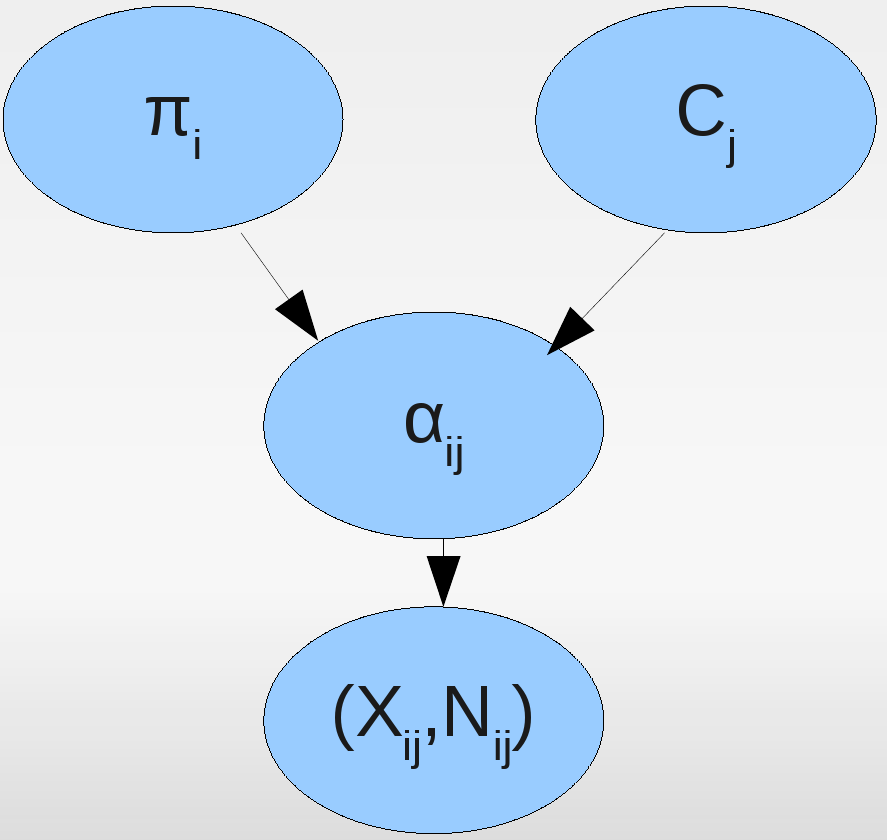
\includegraphics[width=0.2\textwidth]{nicholson-model}
\begin{enumerate}
\item $\alpha^t = P(\alpha|c^{t-1},\pi^{t-1},x)$
\item $\pi^t = P(\pi|c^{t-1},\alpha^t,a)$
\item $c^t = P(c|\pi^t,\alpha^t)$
\end{enumerate}
\item Implemented using a Gibbs sampler in a FORTRAN program.
\item Run on each simulation, and each subset of loci (all,
  not.all.fixed, none.fixed), independently.
}

\picframe{generations-populations}
\picframe{popsize-pneutral}
\picframe{pi-neutral-fixed}
\picframe{pi-error-fixed}
\picframe{ppp}
\picframe{ppp-s}

\framet{Next steps}{
\item Try more focused simulations, smaller number of distinct $s$ values, more replications.
\item Examine distribution of $\hat{c_j}$.
\item Examine distribution of end allele frequencies and fixation,
  conditional on initial population allele frequencies and selection
  parameter $s_i$.
\item Trace false positive and false negative curves using a simple
  ppp-value cutoff rule.
\item Introduce model parameters for selection (Nicholson model
  assumes only drift).
  }

\end{document}